\chapter{Metodologie}\label{chapter:metodologie}
Questo capitolo esplora il ruolo fondamentale del linguaggio ForgeScript, il linguaggio di scripting del rule engine Forge. Saranno analizzate le caratteristiche distintive del linguaggio di ForgeScript, evidenziandone la flessibilità e la potenza espressiva, e verrà presentato il nuovo linguaggio di scripting Lunar, progettato per migliorare la leggibilità e la gestione degli effetti complessi. Infine, sarà esaminato il processo strategico di addestramento dei LLM, attraverso l'impiego di tecniche avanzate come PEFT \cite{peft} e QLoRA \cite{dettmers2023qlora}, al fine di perfezionare la generazione automatica degli script per le carte in uscita nelle nuove espansioni.


\section{Linguaggio a dominio specifico (DSL)}\label{sec:dsl}
Un \emph{linguaggio a dominio specifico} (DSL) è un linguaggio di programmazione o di scripting progettato per un ambito particolare di problemi o applicazioni, come nel nostro caso, i giochi di carte collezionabili. A differenza dei linguaggi di programmazione general-purpose, che sono progettati per essere utilizzati in una vasta gamma di contesti, un DSL è ottimizzato per risolvere problemi specifici all'interno di un determinato dominio.

I vantaggi di utilizzare un DSL includono una maggiore espressività, una maggiore facilità di utilizzo da parte degli utenti nel contesto specifico e la possibilità di incorporare concetti e astrazioni rilevanti per il dominio di interesse. Inoltre, i DSL possono semplificare lo sviluppo e la manutenzione del codice, in quanto sono progettati per risolvere problemi specifici e non includono funzionalità superflue \cite{fowler-dsl}.

\section{Extended Backus-Naur Form (EBNF)}\label{sec:ebnf}
EBNF (o \textit{Extended Backus-Naur Form}) è una notazione formale utilizzata per descrivere la sintassi di un linguaggio di programmazione o di un linguaggio di marcatura. È basata sulla forma originale, la Backus-Naur Form (BNF), ma estende le sue capacità per includere una maggiore espressività.

Nella pratica, EBNF viene utilizzata per definire le regole grammaticali di un linguaggio, specificando come le varie parti del linguaggio possono essere combinate per formare espressioni valide. Le regole sono scritte in forma di produzioni, che indicano come combinare i simboli terminali e non terminali per formare costrutti validi nel linguaggio. Ad esempio, una regola EBNF potrebbe definire che un'espressione matematica può essere composta da un numero seguito da un operatore seguito da un altro numero \cite{feynman2016ebnf}.

\section{Il linguaggio di scripting di Forge}\label{sec:forgescript}
Forge utilizza un linguaggio di scripting di nome ForgeScript, ideato dalla community di sviluppatori che contribuiscono al progetto. ForgeScript utilizza una sintassi che descrive le proprietà delle carte attraverso una struttura chiave-valore, la parte più complessa appare nella parte focale della carta, ovvero i suoi effetti, in cui vengono descritte delle variabili (\textbf{SVars} \cite{forge_api}) per identificare gli effetti da chiamare nella livello core del progetto. Il linguaggio non è compilato, ma consiste in un file con estensione \emph{.txt}, che viene letto da un Parser e ne riconosce le funzioni da chiamare all'interno del livello definito \emph{core}. Questo approccio fornisce la possibilità di poter cambiare il comportamento dello scirpt a runtime, dando un vantaggio agli sviluppatori in fase di Debug. ForgeScript  presenta anche delle problematiche per quanto concerne la leggibilità e la gestione degli effetti delle carte più complesse. Considerando la carta in Figura \ref{fig:lightning_helix} per quanto il suo effetto sia tra i più semplici, è un ottimo esempio per capire come il suo equivalente di ForgeScript sia meno intuitivo.

\begin{figure}
	\centering
	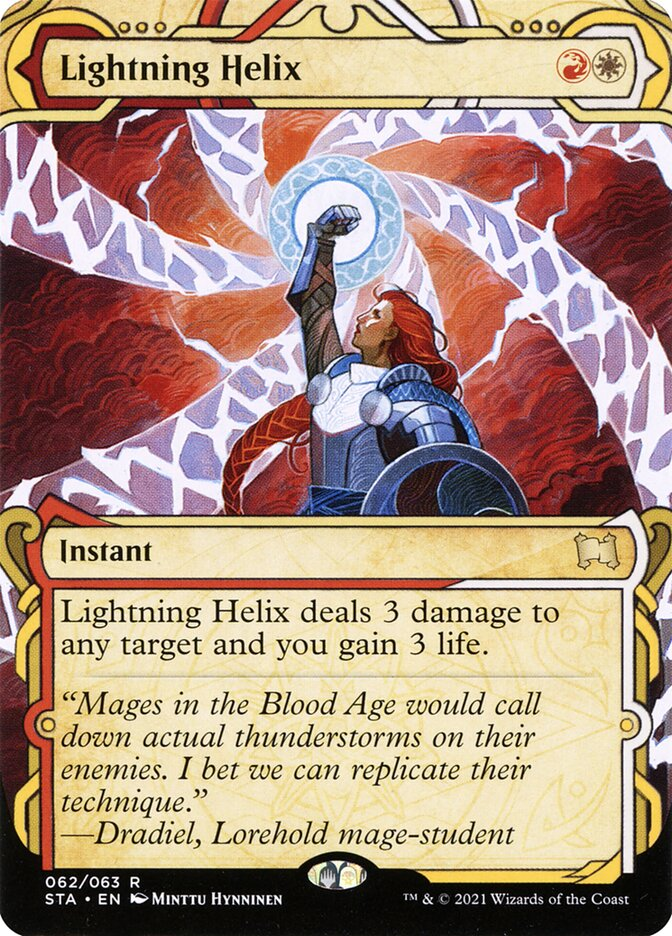
\includegraphics[width=0.6\textwidth]{Immagini/sta-62-lightning-helix.jpg}
	\caption{Carta Lightning Helix con layout Full Art}
	\label{fig:lightning_helix}
\end{figure}
La carta in se permette di infliggere 3 danni ad un qualsiasi bersaglio e di guadagnare 3 punti vita. La risoluzione dei due effetti semplici avviene contemporaneamente, ma prendendo in considerazione lo script descritto dall'Algoritmo \ref{lst:lightning_helix_fs}, si può notare come per un effetto semplice si debba creare una variabile che contenga un sotto effetto per guadagnare vita.

\begin{algorithm}
	\caption{Script della carta in Figura \ref{fig:lightning_helix} in ForgeScript}
	\label{lst:lightning_helix_fs}
	\begin{lstlisting}
Name:Lightning Helix
ManaCost:R W
Types:Instant
A:SP$ DealDamage | Cost$ R W | ValidTgts$ Any | NumDmg$ 3 | SubAbility$ DBGainLife | SpellDescription$ CARDNAME deals 3 damage to any target and you gain 3 life.
SVar:DBGainLife:DB$ GainLife | LifeAmount$ 3
Oracle:Lightning Helix deals 3 damage to any target and you gain 3 life.
	\end{lstlisting}
\end{algorithm}


\section{Lunar, un nuovo linguaggio}\label{sec:lunar_dsl}


Lunar nasce dall'idea di sviluppare un nuovo motore di regole per la gestione delle carte nei giochi di carte collezionabili, fornendo il proprio linguaggio di scripting dedicato. Si ispira alla struttura dei file YAML per rendere l'interazione con il linguaggio più accessibile e intuitiva. L'obiettivo di Lunar è risolvere le limitazioni riscontrate nell'utilizzo di ForgeScript, garantendo una maggiore leggibilità e semplificando la gestione degli effetti complessi all'interno del contesto dei giochi di carte collezionabili.


Di seguito, è presentato come potrebbe apparire la struttura di una carta  di \emph{Magic} scritta in Lunar.

\begin{algorithm}[ht]
	\caption{Struttura di una carta usando Lunar espressa in EBNF}
	\label{lst:ebnf_card}
	\begin{lstlisting}
<card> := <name> <new_line>
          <mana_cost> <new_line>
          <layout> <new_line> 
          <card_type_statement> <new_line> 
          <subtype_statement> <new_line>
          [ <supertype_statement> <new_line> ]
          [ <keywords> ]
          [ <effects> ]
          [ <oracle_text> <new_line>]
          [ <faces> <new_line>]
          [ <power> <new_line>]
          [ <toughness> <new_line>]
          [ <loyalty> <new_line>]
          [ <defence> <new_line>];
	\end{lstlisting}
\end{algorithm}
La seguente grammatica (Algorimo \ref{lst:ebnf_card}) definisce i diversi elementi che compongono una carta, come il nome, il costo di mana, il tipo di carta, le abilità, gli effetti e così via. Questa struttura fornisce una guida su come scrivere correttamente il codice di una carta usando Lunar, garantendo coerenza e uniformità nella sua definizione.
Questi elementi sono rappresentati come regole grammaticali distinte, ciascuna delle quali è seguita da una nuova riga e da un'indentazione per garantire una maggiore leggibilità .

\begin{algorithm}[ht]
	\caption{Struttura di effetto di una carta usando Lunar espressa in EBNF}
	\label{lst:ebnf_effect}
	\begin{lstlisting}
<effects> := `effects: ' <new_line>
                      effect_collection;
<keyword> := `type: ' ( `simple' 
                      | `with_amount' 
                      | `with_amount_and_type' 
                      | `with_cost' 
                      | `with_cost_and_type' 
                      | `with_cost_and_amount'
                      | `with_type' ) <new_line>
              `name: ' keyword_name new_line
              [ `cost: ' {complete_cost}+ <new_line>]
              [ `amount: ' <number> <new_line>]
              [ `affected_type: ' ( <supertype> 
                                  | <card_type> 
                                  | <subtype> ) 
                                 <new_line> ];
         
<effect_collection> :=  {<indent>}+ ( <activated_ability> 
                                    | <base_ability>
                                    | <complex_ability> ) 
                        <new_line> 
                        {effect_collection};
    \end{lstlisting}
\end{algorithm}

Successivamente, la grammatica definisce la struttura degli effetti di una carta, che possono essere di diversi tipi come abilità attivabili, abilità di base o abilità complesse. Ogni tipo di effetto è rappresentato come una raccolta di effetti, ognuno dei quali può essere composto da vari componenti come il tipo di effetto, il nome, il costo, la quantità e il tipo di carta interessata (Algorimo \ref{lst:ebnf_effect}).

Di seguito viene riportato il codice scritto in Lunar della carta in Figura \ref{fig:lightning_helix}:

\begin{algorithm}[ht]
	\caption{Script della carta in Figura \ref{fig:lightning_helix} in Lunar}
	\label{lst:lightning_helix_ln}
	\begin{lstlisting}
name: Lightning Helix
mana_cost: R W
card_type: instant
effects:
    effect:
        type: base
        mode: damage
        target: any_target
        amount: 3
    effect:
        type: base
        mode: life_gain
        target: card_owner
        amount: 3
oracle_text: <Lightning Helix deals 3 damage to any target and you gain 3 life.>
	\end{lstlisting}
\end{algorithm}




Ora proviamo a mettere a confronto come la carta ``Primeval Titan" (vista in Figura \ref{fig:one}) possa essere scritta nel linguaggio ForgeScript e Lunar.


Nel linguaggio ForgeScript, l'implementazione della carta è definita tramite una serie di specifiche riguardanti il nome, il costo di mana, il tipo di carta, le abilità e gli effetti, tutto all'interno di un formato dettagliato e strutturato. Le regole e le azioni sono espresse in modo più verboso e dettagliato, delineando chiaramente le condizioni e gli effetti associati all'entrata in gioco o all'attacco della carta ``Primeval Titan".


\begin{algorithm}
	\caption{Esempio della carta in Figura \ref{fig:one} in ForgeScript}
	\label{lst:prime_titan_fs}
	\begin{lstlisting}
Name:Primeval Titan
ManaCost:4 G G
Types:Creature Giant
PT:6/6
K:Trample
T:Mode$ ChangesZone | Origin$ Any | Destination$ Battlefield | ValidCard$ Card.Self | Execute$ TrigChange | OptionalDecider$ You | TriggerDescription$ Whenever CARDNAME enters the battlefield or attacks, you may search your library for up to two land cards, put them onto the battlefield tapped, then shuffle.
T:Mode$ Attacks | ValidCard$ Card.Self | Execute$ TrigChange | TriggerZones$ Battlefield | OptionalDecider$ You | Secondary$ True | TriggerDescription$ Whenever CARDNAME enters the battlefield or attacks, you may search your library for up to two land cards, put them onto the battlefield tapped, then shuffle.
SVar:TrigChange:DB$ ChangeZone | Origin$ Library | Destination$ Battlefield | Tapped$ True | ChangeType$ Land | ChangeNum$ 2 | ShuffleNonMandatory$ True
SVar:HasAttackEffect:TRUE
Oracle:Trample\nWhenever Primeval Titan enters the battlefield or attacks, you may search your library for up to two land cards, put them onto the battlefield tapped, then shuffle. 
	\end{lstlisting}
\end{algorithm}


\begin{algorithm}
	\caption{Esempio della carta in Figura \ref{fig:one} in Lunar}
	\label{lst:prime_titan_lunar}
	\begin{lstlisting}
name: Primeval Titan
mana_cost: 4 G G
layout: single_face 
card_type: creature
subtype: giant
keywords: 
    keyword:
        type: simple
        name: trample
effects:
    effect:
        type: trigger
        event:
            mode: change_zone
            who: self
            from: anywhere
            to: battlefield
            optional_choice: yes
            optional_decider: card_owner
        event:
            mode: attack
            who: self
            optional_choice: yes
        effect:
            type: base
            mode: move
            from: library
            to: battlefield
            target: land
            amount: 2
            how: tapped
        effect:
            base:
            mode: shuffle
            target: library
oracle_text: <Trample\nWhenever Primeval Titan enters the battlefield or attacks, you may search your library for up to two land cards, put them onto the battlefield tapped, then shuffle.>
power: 6
toughness: 6
	\end{lstlisting}
\end{algorithm}


In contrasto, l'approccio Lunar offre una sintassi più concisa e strutturata, utilizzando un formato ispirato alla leggibilità dei file YAML. La carta è definita in modo più diretto, con chiavi e valori organizzati in una struttura gerarchica. Le abilità e gli effetti sono suddivisi in modo logico, con una chiara distinzione tra eventi come l'entrata in gioco e l'attacco, e le azioni associate ad essi. Questo approccio più compatto rende il codice Lunar più leggibile e facile da comprendere per gli sviluppatori e gli utenti.

In conclusione, sebbene entrambi gli script definiscano la stessa carta, Lunar si distingue per la sua sintassi più pulita e intuitiva, che può rendere il processo di sviluppo e comprensione delle regole del gioco più efficiente e accessibile.
       


\section{QLoRa e PEFT}\label{sec:qlora_peft}


